\newpage
\section{Concurrencia}


\subsection{Concurrencia de Cevianas}


\begin{figure}[htb]
    \centering
    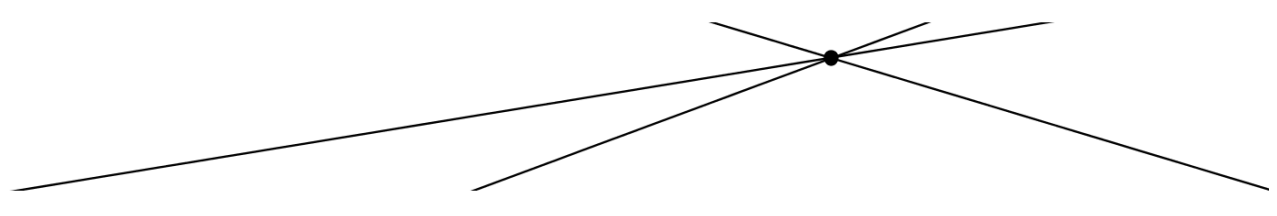
\includegraphics[width=14cm]{images/concurrence-1}
\end{figure}

Tres rectas son concurrentes si pasan por un punto común.
Sabiendo esto, veamos el primer hecho fundamental para abordar los problemas de concurrencia.

\begin{section-theorem.tcb}{Teorema de Ceva}{}
    Dado un triángulo $ABC$, sean $D$, $E$ y $F$ puntos sobre los lados $BC$, $CA$ y $AB$ (o sus prolongaciones), respectivamente.
    Entonces las rectas $AD$, $BE$ y $CF$ son concurrentes si y sólo si
    \begin{gather*}
        \frac{BD}{DC} \cdot \frac{CE}{EA} \cdot \frac{AF}{FB} = 1.
    \end{gather*}
\end{section-theorem.tcb}

A partir de este teorema se vuelve evidente la concurrencia de las principales rectas notables\footnote{Ver los ejercicios del 2.1 al 2.4.}.
De igual forma muchos otros problemas pueden ser resueltos por el teorema de Ceva, la dificultad radica en transformar las proporciones evidentes en otras que sean más fáciles de manipular para que el producto de todas sea igual a 1.

Es importante resaltar que la manipulación de razones con áreas no funciona, pues a partir de la manipulación de áreas también puede ser demostrado este teorema, y lo único que se obtendría es un avanze circular, por ello es mejor hacerlo con semejanza de triángulos, potencia de punto o trigonometría como se verá más adelante.

\begin{section-definition.tcb}{Ceviana}{}
    A toda recta que parte del vértice hacia el lado opuesto se le denomina \textit{ceviana.}
\end{section-definition.tcb}

\begin{section-definition.tcb}{Triángulo ceviano}{}
    Para todo punto $P$, las cevianas desde $A$, $B$ y $C$ que pasan por $P$ y cortan a los lados opuestos en $A'$, $B'$ y $C'$.
    El triángulo $A'B'C'$ es el triángulo ceviano de $P$ y sus vértices se llaman trazas cevianas de $P$.
\end{section-definition.tcb}

\begin{section-theorem.tcb}{Ceva trigonométrico}{}
    Las rectas $AD$, $BE$ y $CF$ son cevianas concurrentes del triángulo $ABC$ si y sólo si
    \begin{gather*}
        \frac{sen(\angle BAD)}{sen(\angle DAC)} \cdot \frac{sen(\angle CBE)}{sen(\angle EBA)} \cdot \frac{sen(\angle ACF)}{sen(\angle FCB)} = 1.
    \end{gather*}
\end{section-theorem.tcb}

La manipulación trigonométrica del teorema de Ceva se vuelve muy importante a la hora de enfrentarse a problemas que pueden parecer práticamente inaccesibles, pues es más general y más aplicable que la semajanza de triángulos.

\begin{section-definition.tcb}{El punto de Gergonne}{}
    Sea $ABC$ un triángulo, y sean $D$, $E$ y $F$ los puntos de tangencia del incírculo con $BC$, $CA$ y $AB$, respectivamente.
    Entonces, $AD$, $BE$ y $CF$ son concurrentes.
\end{section-definition.tcb}

\begin{section-definition.tcb}{El punto de Nagel}{}
    Sea $ABC$ un triángulo, y sean $D'$, $E'$ y $F'$ los puntos de tangencia de los excírculos respectivos a $A$, $B$ y $C$ con $BC$, $CA$ y $AB$, respectivamente.
    Entonces, $AD'$, $BE'$ y $CF'$ son concurrentes.
\end{section-definition.tcb}


\begin{section-theorem.tcb}{Teorema de Ceva sobre la circunferencia}{}
    Sean $ABC$ y $DEF$ dos triángulos sobre la misma circunferencia.
    Entonces las rectas $AD$, $BE$ y $CF$ son concurrentes si y sólo si
    \[\frac{BD}{DC} \cdot \frac{CE}{EA} \cdot \frac{AF}{FB} = 1.\]
\end{section-theorem.tcb}

\begin{section-definition.tcb}{Triángulo circunceviano}{}
    A todo punto que no esté sobre alguno de los lados de un triángulo dado es posible asignarle un nuevo triángulo, que surge a partir de la intersección de las cevianas con el circuncírculo del triángulo.
\end{section-definition.tcb}

\begin{section-theorem.tcb}{Teorema de Steinbart}{}
    Sea $ABC$ un triángulo, $D$, $E$ y $F$ los puntos de tanagencia del incírculo con los lados $BC$, $CA$ y $AB$, respectivamente.
    Sean $P$, $Q$ y $R$ puntos sobre el incírculo de $ABC$.
    Llamemos $A'$, $B'$ y $C'$ las intersecciones de $EF$ con $PD$, $DF$ con $QE$ y $DE$ con $FR$.
    Entonces $AP$, $BQ$ y $CR$ son concurrentes si y sólo si $DP$, $EQ$ y $FR$ son concurrentes.
\end{section-theorem.tcb}

\begin{section-theorem.tcb}{Teorema de Jacobi}{}
    Sea $ABC$ un triángulo, y sean $X$, $Y$, $Z$ tres puntos en el plano tales que $\angle YAC = \angle BAZ$, $\angle ZBA = \angle CBX$, $\angle XCB = \angle ACY$.
    Entonces las rectas $AX$, $BY$ y $CZ$ son concurrentes.
\end{section-theorem.tcb}

\begin{section-definition.tcb}{Puntos isotómicos}{}
    Dos puntos son isotómicos si estos coinciden al ser reflejados por el punto medio del segmento al que pertenecen.
\end{section-definition.tcb}

\begin{section-definition.tcb}{Conjugados isotómicos}{}
    Dado un triángulo $ABC$ se tienen tres cevianas $AD$, $BE$ y $CF$ las cuales son concurrentes en un punto $P$.
    Sean $D'$, $E'$ y $F'$ las reflexiones de $D$, $E$ y $F$ sobre los puntos medios de $BC$, $CA$ y $AB$ respectivamente.
    Entonces las rectas $AD'$, $BE'$ y $CF'$ son concurrentes.
\end{section-definition.tcb}

\begin{section-definition.tcb}{Cevianas isogonales}{}
    Dos cevianas son isogonales del $\triangle ABC$ si ambas parte del mismo vértice del triángulo y una es la reflexión de la otra con respecto a la bisectriz interna de $\triangle ABC$.
\end{section-definition.tcb}

\begin{section-definition.tcb}{Conjugados isogonales}{}
    Dado un triángulo $ABC$ se tienen tres cevianas $AD$, $BE$ y $CF$ las cuales son concurrentes en un punto $P$.
    Sean $AD'$, $BE'$ y $CF'$ las reflexiones de $AD$, $BE$ y $CF$ sobre las bisectrices de $\angle A$, $\angle B$ y $\angle C$ respectivamente.
    Entonces las rectas $AD'$, $BE'$, $CF'$ son concurrentes.
\end{section-definition.tcb}


\begin{section-theorem.tcb}{Steiner}{steiner-theorem}
    Sean $D$ y $E$ dos puntos sobre el segmento $BC$ del triángulo $ABC$ tal que $\angle BAE = \angle DAC$.
    Así
    \[
        \frac{BD}{CD} \cdot \frac{BE}{CE} = \left(\frac{AB}{AC}\right)^2.
    \]
\end{section-theorem.tcb}

\begin{figure}[H]
    \centering
    \definecolor{qqwwcc}{rgb}{0,0.4,0.8}

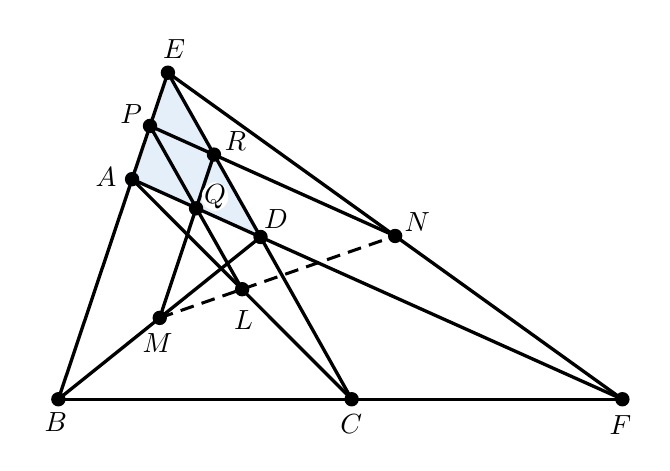
\begin{tikzpicture}[scale = 0.65]
    \clip(-1.86,-1.14) rectangle (10.13,6.98);
    \fill[line width=0pt,color=qqwwcc,fill=qqwwcc,fill opacity=0.1] (0.88,6.1) -- (0.18,4.02) -- (2.69,2.89) -- cycle;
    \draw [line width=1.2pt] (-1.26,-0.28)-- (0.18,4.02);
    \draw [line width=1.2pt] (4.47,-0.28)-- (2.69,2.89);
    \draw [line width=1.2pt] (2.69,2.89)-- (0.18,4.02);
    \draw [line width=1.2pt] (-1.26,-0.28)-- (9.76,-0.28);
    \draw [line width=1.2pt] (2.69,2.89)-- (9.76,-0.28);
    \draw [line width=1.2pt] (2.69,2.89)-- (0.88,6.1);
    \draw [line width=1.2pt] (0.18,4.02)-- (0.88,6.1);
    \draw [line width=1.2pt] (0.88,6.1)-- (9.76,-0.28);
    \draw [line width=1.2pt] (-1.26,-0.28)-- (2.69,2.89);
    \draw [line width=1.2pt] (0.18,4.02)-- (4.47,-0.28);
    \draw [line width=1.2pt] (0.53,5.06)-- (2.33,1.87);
    \draw [line width=1.2pt] (1.78,4.5)-- (0.72,1.31);
    \draw [line width=1.2pt] (0.53,5.06)-- (5.32,2.91);
    \draw [line width=1.1pt,dash pattern=on 5pt off 3pt] (0.72,1.31)-- (5.32,2.91);
    \begin{scriptsize}
        \normalsize
        \fill [color=black] (0.18,4.02) circle (4.0pt);
        \draw[color=black] (-0.33,4.06) node {$A$};
        \fill [color=black] (-1.26,-0.28) circle (4.0pt);
        \draw[color=black] (-1.31,-0.73) node {$B$};
        \fill [color=black] (4.47,-0.28) circle (4.0pt);
        \draw[color=black] (4.46,-0.76) node {$C$};
        \fill [color=black] (2.69,2.89) circle (4.0pt);
        \draw[color=black] (2.99,3.25) node {$D$};
        \fill [color=black] (0.88,6.1) circle (4.0pt);
        \draw[color=black] (1,6.57) node {$E$};
        \fill [color=black] (9.76,-0.28) circle (4.0pt);
        \draw[color=black] (9.72,-0.78) node {$F$};
        \fill [color=black] (0.72,1.31) circle (4.0pt);
        \draw[color=black] (0.68,0.82) node {$M$};
        \fill [color=black] (2.33,1.87) circle (4.0pt);
        \draw[color=black] (2.36,1.26) node {$L$};
        \fill [color=black] (1.43,3.45) circle (4.0pt);
        \draw[color=black] (1.8,3.68) node[fill = white, rounded corners = 5pt, inner sep=0.8pt] {$Q$};
        \fill [color=black] (0.53,5.06) circle (4.0pt);
        \draw[color=black] (0.16,5.29) node {$P$};
        \fill [color=black] (1.78,4.5) circle (4.0pt);
        \draw[color=black] (2.2,4.77) node[fill = white, rounded corners = 5pt, inner sep=0.8pt] {$R$};
        \fill [color=black] (5.32,2.91) circle (4.0pt);
        \draw[color=black] (5.75,3.19) node {$N$};
    \end{scriptsize}
\end{tikzpicture}
\end{figure}

\begin{proof}
    Aplicando el~\refTheorem{\ref{t:ratio-lemma}} al $\triangle ABC$ con los puntos $D$ y $E$, respectivamente, se obtiene:
    \begin{align*}
        \frac{BD}{DC} = \frac{AB}{AC} \cdot \frac{\sen(\angle BAD)}{\sen(\angle DAC)} \quad \land \quad
        \frac{BE}{EC} = \frac{AB}{AC} \cdot \frac{\sen(\angle BAE)}{\sen(\angle EAC)} \\[3mm]
        \implies \frac{BD}{DC} \cdot \frac{BE}{EC} = \left(\frac{AB}{AC}\right)^2 \cdot \frac{\sen(\angle BAD)}{\sen(\angle DAC)} \cdot \frac{\sen(\angle BAE)}{\sen(\angle EAC)}
    \end{align*}
    Pero como $\angle BAE = \angle DAC$, entonces $\angle BAD = \angle EAC$, de donde se sigue el resultado.
\end{proof}


\subsection{Simedianas}

\begin{section-definition.tcb}{Simediana}{}
    La simediana correspondiente al vértice $A$ se define como la reflexión de $A$\nobreakdash-mediana con respecto a la bisectriz interna del ángulo $\angle BAC$.
    En otras palabras, es la recta isogonal correspondiente a la mediana que parte del mismo vértice de referencia.
\end{section-definition.tcb}

\begin{figure}[H]
    \centering
    \begin{tikzpicture}[xscale = 1.5, yscale = 1.5]

\end{tikzpicture}
    \caption{La recta $AL$ es la $A$-simediana del triángulo $ABC$.}
    \label{fig:symmedian-definition}
\end{figure}

En el caso de la figura~\ref{fig:symmedian-definition}, la recta $AL$ es la $A$-simediana del $\triangle ABC$.
Es decir $\angle BAL = \angle MAC$.
No hace falta decir que todo triángulo contiene tres simedianas.
Por la \refDefinition{1.4} vista en la clase anterior, sabemos que, al concurrir las medianas en el baricentro, las simedianas comparten también un punto en común, llamado el \textbf{punto de Lemoine}.


\begin{section-lemma.tcb}{}{symmendian-proportion}
    Sea $N$ un punto sobre el segmento $BC$; entonces, $N$ pertenece a la $A$\nobreakdash-simediana si y solo si
    \[
        \frac{BN}{NC} = \left(\frac{AB}{AC}\right)^2.
    \]
\end{section-lemma.tcb}

\begin{proof}
    Es una aplicación directa del~\refTheorem{\ref{t:steiner-theorem}}.
\end{proof}


\begin{section-lemma.tcb}{}{simedian-lemma}
    Sea $D$ el punto de intersección de las tangentes por $B$ y $C$ al circuncírculo del triángulo $ABC$.
    Luego, $AD$ es una simediana de $\triangle ABC$.
\end{section-lemma.tcb}

\begin{proof}
    Supongamos que las prolongaciones de los lados $AB$ y $AC$ cortan a la paralela a $BC$ por $P$ en $S$ y $T$, respectivamente.
    Es claro que $\angle PSB = \angle CBA$ y $\angle PTC = \angle BCA$.
    Además, $\angle PBS = \angle BCA$ y $\angle PCT = \angle CBA$ por la condición de tangencia de $PB$ y $PC$.

    \begin{figure}[H]
        \centering
        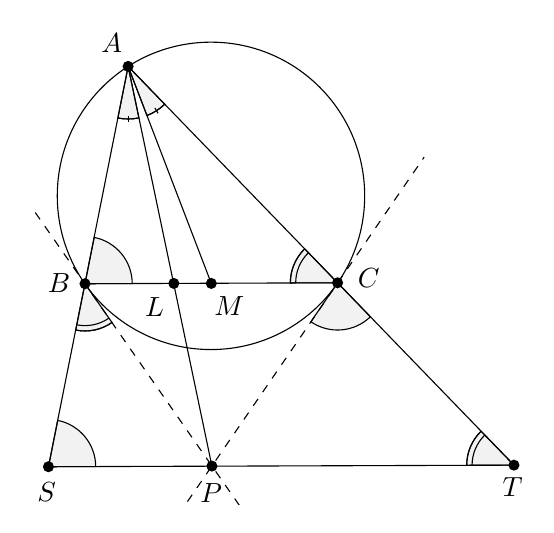
\begin{tikzpicture}[scale = 0.4]
    \clip(-2.36,-10.08) rectangle (13.47,5.06);
    \draw [shift={(-0.54,-3.07)},fill=black,fill opacity=0.05] (0,0) -- (0.2:1.5) arc (0.2:78.71:1.5) -- cycle;
    \draw [shift={(7.48,-3.04)},fill=black,fill opacity=0.05] (0,0) -- (-124.46:1.5) arc (-124.46:-45.95:1.5) -- cycle;
    \draw [shift={(-1.7,-8.88)},fill=black,fill opacity=0.05] (0,0) -- (0.2:1.5) arc (0.2:78.71:1.5) -- cycle;
    \draw [shift={(-0.54,-3.07)},fill=black,fill opacity=0.05] (0,0) -- (-101.29:1.5) arc (-101.29:-55.14:1.5) -- cycle;
    \draw [shift={(7.48,-3.04)},fill=black,fill opacity=0.05] (0,0) -- (134.05:1.5) arc (134.05:180.2:1.5) -- cycle;
    \draw [shift={(13.08,-8.83)},fill=black,fill opacity=0.05] (0,0) -- (134.05:1.5) arc (134.05:180.2:1.5) -- cycle;
    \draw [shift={(0.83,3.83)},fill=black,fill opacity=0.05] (0,0) -- (-101.29:1.67) arc (-101.29:-78.18:1.67) -- cycle;
    \draw [shift={(0.83,3.83)},fill=black,fill opacity=0.05] (0,0) -- (-69.06:1.67) arc (-69.06:-45.95:1.67) -- cycle;
    \draw(3.46,-0.28) circle (4.88cm);
    \draw (-0.54,-3.07)-- (7.48,-3.04);
    \draw (0.83,3.83)-- (-1.7,-8.88);
    \draw (0.83,3.83)-- (13.08,-8.83);
    \draw (-1.7,-8.88)-- (13.08,-8.83);
    \draw (0.83,3.83)-- (3.49,-8.86);
    \draw (0.83,3.83)-- (3.47,-3.06);
    \draw [dash pattern=on 3pt off 3pt,domain=-2.1176316762214267:13.472829432059696] plot(\x,{(-21.59-8.05*\x)/5.61});
    \draw [dash pattern=on 3pt off 3pt,domain=-2.361745286484902:10.226227746616733] plot(\x,{(--93.93-9.81*\x)/-6.74});
    \draw [shift={(-0.54,-3.07)}] (-101.29:1.5) arc (-101.29:-55.14:1.5);
    \draw [shift={(-0.54,-3.07)}] (-101.29:1.33) arc (-101.29:-55.14:1.33);
    \draw [shift={(7.48,-3.04)}] (134.05:1.5) arc (134.05:180.2:1.5);
    \draw [shift={(7.48,-3.04)}] (134.05:1.33) arc (134.05:180.2:1.33);
    \draw [shift={(13.08,-8.83)}] (134.05:1.5) arc (134.05:180.2:1.5);
    \draw [shift={(13.08,-8.83)}] (134.05:1.33) arc (134.05:180.2:1.33);
    \draw [shift={(0.83,3.83)}] (-101.29:1.67) arc (-101.29:-78.18:1.67);
    \draw(0.84,2.27) -- (0.84,2.07);
    \draw [shift={(0.83,3.83)}] (-69.06:1.67) arc (-69.06:-45.95:1.67);
    \draw(1.68,2.51) -- (1.78,2.34);
    \begin{scriptsize}
        \normalsize
        \fill [color=black] (0.83,3.83) circle (5pt);
        \draw[color=black] (0.31,4.56) node {$A$};
        \fill [color=black] (3.49,-8.86) circle (5pt);
        \draw[color=black] (3.47,-9.7) node {$P$};
        \fill [color=black] (-0.54,-3.07) circle (5pt);
        \draw[color=black] (-1.36,-3.04) node {$B$};
        \fill [color=black] (7.48,-3.04) circle (5pt);
        \draw[color=black] (8.47,-2.88) node {$C$};
        \fill [color=black] (-1.7,-8.88) circle (5pt);
        \draw[color=black] (-1.76,-9.68) node {$S$};
        \fill [color=black] (13.08,-8.83) circle (5pt);
        \draw[color=black] (13.04,-9.54) node {$T$};
        \fill [color=black] (2.28,-3.06) circle (5pt);
        \draw[color=black] (1.67,-3.81) node {$L$};
        \fill [color=black] (3.47,-3.06) circle (5pt);
        \draw[color=black] (4.04,-3.78) node {$M$};
    \end{scriptsize}
\end{tikzpicture}
        \caption{Una forma de construir e identificar la $A$-simediana.}
    \end{figure}

    De este modo, $\triangle BPS \sim \triangle CAB \sim \triangle TPC$, lo que a su vez implica que:
    \begin{align*}
        \frac{SP}{PB} = \frac{AB}{AC} \ \land \ \frac{PC}{PT} = \frac{AB}{AC}
        \ \implies \ \frac{SP}{PB} \cdot \frac{PC}{PT} &= \left(\frac{AB}{AC}\right)^2\\
        \frac{SP}{PB} \cdot \frac{PC}{PT} &= \left(\frac{AS}{AT}\right)^2 \quad \text{(Por $\triangle CAB \sim \triangle TAS$)}\\
        \frac{SP}{PT}  &= \left(\frac{AS}{AT}\right)^2 \quad \text{($PB = PC$ por tangencia)}
    \end{align*}
    luego, por el lema~\ref{l:symmendian-proportion}, $AP$ es simediana de $\triangle SAT$ y, de paso, también de $\triangle BAC$.
\end{proof}


\begin{section-definition.tcb}{Recta de Lemoine}{}
    Sea el triángulo $ABC$ y $\Omega$ su circuncírculo, las tangentes a $\Omega$ por $A$, $B$ y $C$ se intersecan con los lados opuestos $BC$, $AC$ y $BA$ en los puntos $E$, $F$ y $D$, respectivamente.
    Así, se cumple que $E$, $F$ y $D$ están sobre una misma recta, llamada la \textbf{recta de Lemoine} del triángulo $ABC$.
\end{section-definition.tcb}






\subsection{Ejercicios y Problemas}
Sección de ejercicios y problemas para el autoestudio.

\begin{section-exercise}
    Demostrar que todas las medianas de un triángulo concurren en un punto (Baricentro).
\end{section-exercise}

\begin{section-exercise}
    Demostrar que todas las alturas de un triángulo concurren en un punto (Ortocentro).
\end{section-exercise}

\begin{section-exercise}
    Demostrar que todas las bisectrices interiores de un triángulo concurren en un punto (Incentro).
\end{section-exercise}

\begin{section-exercise}
    Demostrar que dos bisectrices exteriores y una bisectriz interior de un triángulo concurren en un punto (Excentro).
\end{section-exercise}

\begin{section-exercise}
    Sean $BE$, $AD$ y $CF$ líneas tales que dividen a un triángulo en $AE = 12$, $EC = 6$, $CD = 7$, $DB = 10$, $BF = 5$, $FA = 7$.
    Demostrar que $BE$, $AD$ y $CF$ son concurrentes.
\end{section-exercise}

\begin{section-exercise}
    Sea $ABC$ un triángulo con lados $AB$, $BC$, $CA$ que tienen longitudes 13, 15, 14, respectivamente.
    Si $CF$, $AD$ y $BE$ concurren y $\dfrac{AF}{FB} = \dfrac{2}{5}$ y $\dfrac{CE}{EA} = \dfrac{5}{8}$, encuentra el valor de $BD$ y $DC$.
\end{section-exercise}

\begin{section-exercise}
    En un triángulo $ABC$ en el cual se traza la altura $BH$, la mediana $AM$ y la ceviana $CN$ las cuales concurren en el punto $P$.
    Si $BP = 3PH$ y $NB = 16$.
    Hallar $AN$.
\end{section-exercise}

\begin{section-exercise}
    Si $P$ y $Q$ son puntos en $AB$ y $AC$ del triángulo $ABC$ de tal forma que $PQ$ es paralelo a $BC$, y si $BQ$ y $CP$ se cortan en $O$, demuestra que $AO$ es una mediana.
\end{section-exercise}

\begin{section-exercise}
    Sean $L$, $M$ y $N$ puntos en los lados $BC$, $CA$ y $AB$ de un triángulo, respectivamente.
    Si $AL$, $BM$ y $CN$ concurren en $O$, demostrar que
    \[\frac{OL}{AL} + \frac{OM}{BM} + \frac{ON}{CN} = 1.\]
\end{section-exercise}

\begin{section-exercise}
    Sean $L$, $M$ y $N$ puntos en los lados $BC$, $CA$ y $AB$ de un triángulo, respectivamente.
    Si $AL$, $BM$ y $CN$ concurren en $O$, demostrar que
    \[\frac{AO}{OL} = \frac{AN}{NB} + \frac{AM}{MC}.\]
\end{section-exercise}


\begin{section-exercise}
    Realizar la construcción de las tres simedianas de un triángulo $ABC$ con la ayuda del Lemma~\ref{l:simedian-lemma} y ubicar el punto de \textbf{Lemoine}.
\end{section-exercise}

\begin{section-exercise}
    Realizar la construcción de la recta de \textbf{Lemoine} para un triángulo $ABC$.
\end{section-exercise}


\begin{section-problem}
    Sea $ABC$ un triángulo.
    Se toman los puntos $D$, $E$ y $F$ en las mediatrices de $BC$, $CA$ y $AB$ respectivamente.
    Probar que las rectas que pasan por $A$, $B$ y $C$ que son perpendiculares a $EF$, $FD$ y $DE$, respectivamente, son concurrentes.
\end{section-problem}

\begin{section-problem}
    Sea $L$ el punto de \textbf{Lemoine} de un triángulo $ABC$ y $M$ el punto en $BC$ tal que $AM$ contiene a $L$.
    Demostrar que
    \[
        \frac{AL}{LM} = \frac{BA^2 + AC^2}{BC^2}.
    \]
\end{section-problem}

\begin{section-problem}
    Las bisectrices interna y externa del ángulo $\angle BAC$ de $\triangle ABC$, intersecan a la recta $BC$ en $E$ y $D$, respectivamente.
    El circuncírculo de $\triangle DEA$ interseca al circuncírculo de $\triangle ABC$ en $X$.
    Probar que $AX$ es la $A$-simediana de $\triangle ABC$.
\end{section-problem}

\begin{section-problem}
    Sea $AD$ una altura de $\triangle ABC$.
    Consideremos $AD$ como diámetro de una circunferencia que corta los $AB$ y $AC$ en $K$ y $L$, respectivamente.
    Las tangentes a la circunferencia en los puntos $K$ y $L$ se intersectan en un punto $M$.
    Demuestra que la recta $AM$ divide $BC$ por la mitad.
\end{section-problem}

\begin{section-problem}
    Un cuadrilátero convexo $ABCD$ tiene $AD = CD$ y $\angle DAB = \angle ABC < 90^\circ$.
    La recta por $D$ y el punto medio de $BC$ intersecta a la recta $AB$ en un punto $E$.
    Demuestra qur $\angle BEC = \angle DAC$.
\end{section-problem}

\begin{section-problem}
    Una recta paralela a $BC$ corta a los lados $AB$ y $AC$ en $M$ y $N$ en el $\triangle ABC$, respectivamente.
    Sea $P$ el punto de corte de $BN$ y $CM$.
    Sea $Q$ el segundo punto de corte de los circuncírculos de $MPB$ y $NCP$.
    Demostrar que $\angle BAQ = \angle PAC$.
\end{section-problem}
